\documentclass{minimal}

\usepackage{tikz}
\usetikzlibrary{trees}

\begin{document}
\tikzstyle{every node}=[draw=black,thick,anchor=west]
\tikzstyle{selected}=[draw=red,fill=red!30]
\tikzstyle{optional}=[dashed,fill=gray!50]
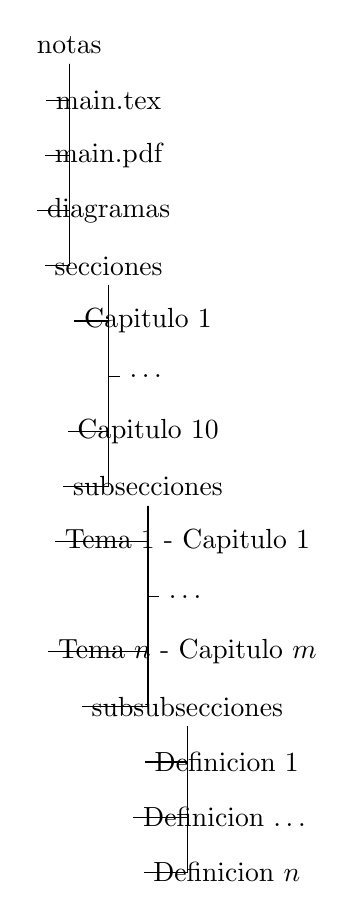
\begin{tikzpicture}[%
  grow via three points={one child at (0.5,-0.7) and
  two children at (0.5,-0.7) and (0.5,-1.4)},
  edge from parent path={(\tikzparentnode.south) |- (\tikzchildnode.west)}]
  \node {notas}
    child { node {main.tex}}		
    child { node {main.pdf}}
    % child { node {source}}
    child { node {diagramas}}
    child { node {secciones}
      child { node {Capitulo 1}}
      child { node {\dots}}
      child { node {Capitulo 10}}
      % child { node [selected] {tex}
      child { node {subsecciones}
        child { node {Tema 1 - Capitulo 1}}
        child { node {\dots}}
        child { node {Tema $n$ - Capitulo $m$}}
        child { node {subsubsecciones}
          child { node {Definicion 1}}
          child { node {Definicion \dots}}
          child { node {Definicion $n$}}
        }
      }
    %   child { node [optional] {latex}}
    };
    child [missing] {}				
    child [missing] {}				
    child [missing] {}				
    % child { node {texdoc}};
\end{tikzpicture}
\end{document}